
%% Hooke Questions used on the
%% NYSED Physics Regents Examination
%%--------------------------------------------------

%% this section contains 13 problems


%% Section June2015
%%--------------------
\element{nysed}{
\begin{question}{June2015-Q06}
    A vertical spring has a spring constant of \SI{100}{\newton\per\meter}.
    When an object is attached to the bottom of the spring,
        the spring changes from its unstretched length of \SI{0.50}{\meter} to a length of \SI{0.65}{\meter}. 
    The magnitude of the weight of the attached object is:
    \begin{multicols}{2}
    \begin{choices}
        \wrongchoice{\SI{1.1}{\newton}}
      \correctchoice{\SI{15}{\newton}}
        \wrongchoice{\SI{50}{\newton}}
        \wrongchoice{\SI{65}{\newton}}
    \end{choices}
    \end{multicols}
\end{question}
}

\element{nysed}{
\begin{question}{June2015-Q43}
    Which graph best represents the relationship between the potential energy stored in a spring and the change in the spring's length from its equilibrium position?
    \begin{multicols}{2}
    \begin{choices}
        \AMCboxDimensions{down=-2.5em}
        \correctchoice{
            \begin{tikzpicture}
                \begin{axis}[
                    axis y line=left,
                    axis x line=bottom,
                    axis line style={->},
                    xlabel={change in length},
                    xtick=\empty,
                    ylabel={potential energy},
                    ytick=\empty,
                    xmin=0,xmax=11,
                    ymin=0,ymax=11,
                    width=1.00\columnwidth,
                    very thin,
                    font=\small,
                ]
                \addplot[line width=1pt,domain=0:10]{0.1*x*x};
                \end{axis}
            \end{tikzpicture}
        }
        \wrongchoice{
            \begin{tikzpicture}
                \begin{axis}[
                    axis y line=left,
                    axis x line=bottom,
                    axis line style={->},
                    xlabel={change in length},
                    xtick=\empty,
                    ylabel={potential energy},
                    ytick=\empty,
                    xmin=0,xmax=11,
                    ymin=0,ymax=11,
                    width=1.00\columnwidth,
                    very thin,
                    font=\small,
                ]
                \addplot[line width=1pt,domain=0:10]{x};
                \end{axis}
            \end{tikzpicture}
        }
        \wrongchoice{
            \begin{tikzpicture}
                \begin{axis}[
                    axis y line=left,
                    axis x line=bottom,
                    axis line style={->},
                    xlabel={change in length},
                    xtick=\empty,
                    ylabel={potential energy},
                    ytick=\empty,
                    xmin=0,xmax=11,
                    ymin=0,ymax=11,
                    width=1.00\columnwidth,
                    very thin,
                    font=\small,
                ]
                \addplot[line width=1pt,domain=0:10]{10-x};
                \end{axis}
            \end{tikzpicture}
        }
        \wrongchoice{
            \begin{tikzpicture}
                \begin{axis}[
                    axis y line=left,
                    axis x line=bottom,
                    axis line style={->},
                    xlabel={change in length},
                    xtick=\empty,
                    ylabel={potential energy},
                    ytick=\empty,
                    xmin=0,xmax=11,
                    ymin=0,ymax=11,
                    width=1.00\columnwidth,
                    very thin,
                    font=\small,
                ]
                \addplot[line width=1pt,domain=0:10]{10/x};
                \end{axis}
            \end{tikzpicture}
        }
    \end{choices}
    \end{multicols}
\end{question}
}


%% Section June2007
%%--------------------
\element{nysed}{
\begin{question}{Jan2009-Q02}
    An unstretched spring has a length of \SI{10}{\centi\meter}.
    When the spring is stretched by a force of \SI{16}{\newton},
        its length is increased to \SI{18}{\centi\meter}.
    What is the spring constant of the spring?
    \begin{multicols}{2}
    \begin{choices}
        \wrongchoice{\SI{0.86}{\newton\per\centi\meter}}
      \correctchoice{\SI{2.0}{\newton\per\centi\meter}}
        \wrongchoice{\SI{1.6}{\newton\per\centi\meter}}
        \wrongchoice{\SI{1.8}{\newton\per\centi\meter}}
    \end{choices}
    \end{multicols}
\end{question}
}


%% Section June2007
%%--------------------
\element{nysed}{
\begin{question}{June2007-Q07}
    The diagram below represents a spring hanging vertically that stretches \SI{0.075}{\meter} when a \SI{5.0}{\newton} block is attached.
    The spring-block system is at rest in the position shown.
    \begin{center}
    \begin{tikzpicture}
        \begin{scope}[xshift=-2cm]
            %% Title
            \node[anchor=south,text centered] at (0.5,0.2cm) {Unstretched};
            %% Celiing
            \draw (-1,0) --  (2,0);
            \node[anchor=south,fill,pattern=north east lines,minimum width=3cm, minimum height=0.05cm] at (0.5,0) {};
            %% Spring
            \draw[thick,decoration={aspect=0.2,segment length=2mm,amplitude=4mm,coil},decorate] (0,0) -- (0,-1.5);
            \draw[dashed]  (0,-1.5) -- ++(0:2.5cm);
        \end{scope}
        \begin{scope}
            \draw[<->,thick] (0,-3) -- (0,-1.5) node[pos=0.5,anchor=center,fill=white] {\SI{0.075}{\meter}};
        \end{scope}
        \begin{scope}[xshift=+2cm]
            %% Title
            \node[anchor=south,text centered] at (0.5,0.2cm) {Stretched};
            %% Celiing
            \draw (-1,0) --  (2,0);
            \node[anchor=south,fill,pattern=north east lines,minimum width=3cm, minimum height=0.05cm] at (0.5,0) {};
            %% Weight
            \node[anchor=north,draw,minimum size=1cm] (M) at (0,-3) {\SI{5}{\newton}};
            %% Spring
            \draw[thick,decoration={aspect=0.2,segment length=3mm,amplitude=4mm,coil},decorate] (0,0) -- (0,-3);
            \draw[dashed]  (0,-3) -- ++(180:2.5cm);
        \end{scope}
    \end{tikzpicture}
    \end{center}
    The value of the spring constant is:
    \begin{multicols}{2}
    \begin{choices}
      \correctchoice{\SI{67}{\newton\per\meter}}
        \wrongchoice{\SI{38}{\newton\per\meter}}
        \wrongchoice{\SI{130}{\newton\per\meter}}
        \wrongchoice{\SI{650}{\newton\per\meter}}
    \end{choices}
    \end{multicols}
\end{question}
}


%% Section June2006
%%--------------------
\element{nysed}{
\begin{question}{June2006-Q39}
    The graph below represents the relationship between the force applied to a spring and spring elongation for four different springs?
    \begin{center}
    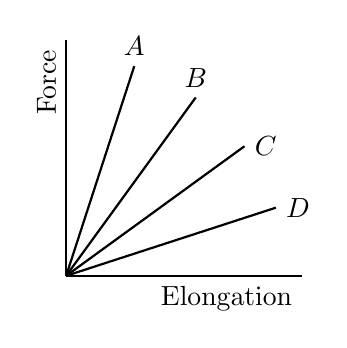
\begin{tikzpicture}
        \draw[thick] (0,0) -- (0,3) node[anchor=south east,rotate=90] {Force};
        \draw[thick] (0,0) -- (3,0) node[anchor=north east] {Elongation};
        \draw[thick] (0,0) -- (72:2.8) node[anchor=south] {$A$};
        \draw[thick] (0,0) -- (54:2.8) node[anchor=south] {$B$};
        \draw[thick] (0,0) -- (36:2.8) node[anchor=west] {$C$};
        \draw[thick] (0,0) -- (18:2.8) node[anchor=west] {$D$};
    \end{tikzpicture}
    \end{center}
    Which spring has the greatest spring constant?
    \begin{multicols}{4}
    \begin{choices}
      \correctchoice{$A$}
        \wrongchoice{$B$}
        \wrongchoice{$C$}
        \wrongchoice{$D$}
    \end{choices}
    \end{multicols}
\end{question}
}


%% Section Jan2006
%%--------------------
\element{nysed}{
\begin{question}{Jan2006-Q09}
    A vertical spring \SI{0.100}{\meter} long is elongated to a length of \SI{0.119}{\meter} when a \SI{1.00}{\kilo\gram} mass is attached to the bottom of the spring.
    The spring constant of this spring is:
    \begin{multicols}{2}
    \begin{choices}
      \correctchoice{\SI{520}{\newton\per\meter}}
        \wrongchoice{\SI{98}{\newton\per\meter}}
        \wrongchoice{\SI{82}{\newton\per\meter}}
        \wrongchoice{\SI{9.8}{\newton\per\meter}}
    \end{choices}
    \end{multicols}
\end{question}
}


%% Section Jan2005
%%--------------------


%% Section June2005
%%--------------------
\element{nysed}{
\begin{question}{June2005-Q11}
    The spring in a scale in the produce department of a supermarket stretches \SI{0.025}{\meter} when a watermelon weighing \SI{1.0e2}{\newton} is placed on the scale.
    The spring constant for this spring is:
    \begin{multicols}{2}
    \begin{choices}
      \correctchoice{\SI{4.0e3}{\newton\per\meter}}
        \wrongchoice{\SI{3.2e5}{\newton\per\meter}}
        \wrongchoice{\SI{2.5}{\newton\per\meter}}
        \wrongchoice{\SI{3.1e-2}{\newton\per\meter}}
    \end{choices}
    \end{multicols}
\end{question}
}


%% Section Jan2003
%%--------------------
\element{nysed}{
\begin{question}{Jan2003-Q46}
    The graph below shows elongation as a function of the applied force for two springs, $A$ and $B$.
    \begin{center}
    \begin{tikzpicture}
        \begin{axis}[
            axis y line=left,
            axis x line=bottom,
            axis line style={->},
            ylabel={elongation},
            y unit=\si{\meter},
            ytick={0,0.10,0.20,0.30},
            xlabel={Force},
            x unit=\si{\newton},
            xtick={0,1.0,2.0,3.0,4.0},
            xmin=0,xmax=4,
            ymin=0,ymax=0.30,
            grid=major,
            width=0.8\columnwidth,
            height=0.5\columnwidth,
            very thin,
        ]
        \addplot[line width=1pt,domain=0:4]{0.1071 * x}
            node[anchor=south east,pos=0.5] {$A$};
        \addplot[line width=1pt,domain=0:4]{0.065 * x}
             node[anchor=south east,pos=0.75] {$B$};
        \end{axis}
    \end{tikzpicture}
    \end{center}
    Compared to the spring constant for spring $A$,
        the spring constant for spring $B$ is:
    \begin{multicols}{3}
    \begin{choices}
        \wrongchoice{smaller}
      \correctchoice{larger}
        \wrongchoice{the same}
    \end{choices}
    \end{multicols}
\end{question}
}


%% Section Jan2002
%%--------------------
\element{nysed}{
\begin{question}{Jan2002-Q21}
    The graph below shows the relationship between the elongation of a spring and the force applied to the spring causing it to stretch.
    \begin{center}
    \begin{tikzpicture}
        \begin{axis}[
            axis y line=left,
            axis x line=bottom,
            axis line style={->},
            ylabel={elongation},
            y unit=\si{\meter},
            ytick={0,0.10,0.20,0.30,0.40,0.50},
            xlabel={Force},
            x unit=\si{\newton},
            xtick={0,5,10,15,20},
            xmin=0,xmax=25,
            ymin=0,ymax=0.52,
            grid=major,
            width=0.8\columnwidth,
            height=0.5\columnwidth,
            very thin,
        ]
        \addplot[line width=1pt,domain=0:25]{0.02*x};
        \end{axis}
    \end{tikzpicture}
    \end{center}
    What is the spring constant for this spring?
    \begin{multicols}{2}
    \begin{choices}
        \wrongchoice{\SI{0.020}{\newton\per\meter}}
        \wrongchoice{\SI{2.0}{\newton\per\meter}}
        \wrongchoice{\SI{25}{\newton\per\meter}}
      \correctchoice{\SI{50}{\newton\per\meter}}
    \end{choices}
    \end{multicols}
\end{question}
}


%% Section Jan2002
%%--------------------
\element{nysed}{
\begin{question}{June2000-Q25}
    The graph below represents the relationship between the force applied to a spring and the compression (displacement) of the spring.
    \begin{center}
    \begin{tikzpicture}
        \begin{axis}[
            axis y line=left,
            axis x line=bottom,
            axis line style={->},
            ylabel={force},
            y unit=\si{\newton},
            ytick={0,0.20,0.40,0.60,0.80,1.00},
            xlabel={compression},
            x unit=\si{\meter},
            xtick={0,0.10,0.20,0.30,0.40},
            xmin=0,xmax=0.45,
            ymin=0,ymax=1.05,
            grid=major,
            width=0.8\columnwidth,
            height=0.5\columnwidth,
            very thin,
        ]
        \addplot[line width=1pt,domain=0:0.45]{2.5*x};
        \end{axis}
    \end{tikzpicture}
    \end{center}
    What is the spring constant for this spring?
    \begin{multicols}{2}
    \begin{choices}
        \wrongchoice{\SI{1.0}{\newton\per\meter}}
      \correctchoice{\SI{2.5}{\newton\per\meter}}
        \wrongchoice{\SI{0.20}{\newton\per\meter}}
        \wrongchoice{\SI{0.40}{\newton\per\meter}}
    \end{choices}
    \end{multicols}
\end{question}
}


%% Section Jan2001
%%--------------------
\element{nysed}{
\begin{question}{Jan2001-Q10}
    %% NOTE: this is a measurement problem
    What is the displacement of the mass hanger ($H$) shown in the diagram after a \SI{0.20}{\kilo\gram} mass is loaded on it?
    [Assume the hanger is at rest in both positions.]
    \begin{center}
        \includegraphics[keepaspectratio,scale=0.75]{Jan2001-Q10}
    \end{center}
    \begin{multicols}{2}
    \begin{choices}
        \wrongchoice{\SI{12.30}{\centi\meter}}
        \wrongchoice{\SI{12.50}{\centi\meter}}
      \correctchoice{\SI{12.70}{\centi\meter}}
        \wrongchoice{\SI{13.30}{\centi\meter}}
    \end{choices}
    \end{multicols}
\end{question}
}


%% Section June1999
%%--------------------

%% NOTE: June1999-Q21 utilizes a possible duplicate (I can change numbers),
%%  or tikz, they are just ovals after all?


%% Section June1997
%%--------------------
\element{nysed}{
\begin{question}{June1997-Q19}
    The graph below shows the relationship between the elongation of a spring and the force applied to the spring causing it to stretch.
    \begin{center}
    \begin{tikzpicture}
        \begin{axis}[
            axis y line=left,
            axis x line=bottom,
            axis line style={->},
            ylabel={elongation},
            y unit=\si{\meter},
            ytick={0,0.10,0.20,0.30,0.40,0.50,0.60},
            ymin=0,ymax=0.62,
            xlabel={Force},
            x unit=\si{\newton},
            xtick={0,10,20,30},
            xmin=0,xmax=30,
            grid=major,
            width=0.8\columnwidth,
            height=0.5\columnwidth,
            very thin,
        ]
        \addplot[line width=1pt,domain=0:30]{0.02*x};
        \end{axis}
    \end{tikzpicture}
    \end{center}
    What is the spring constant for this spring?
    \begin{multicols}{2}
    \begin{choices}
        \wrongchoice{\SI{0.020}{\newton\per\meter}}
        \wrongchoice{\SI{2.0}{\newton\per\meter}}
        \wrongchoice{\SI{25}{\newton\per\meter}}
      \correctchoice{\SI{50}{\newton\per\meter}}
    \end{choices}
    \end{multicols}
\end{question}
}


%% Section June1996
%%--------------------
\element{nysed}{
\begin{question}{June1996-Q20}
    A \SI{20}{\newton} weight is attached to a spring,
        causing it to stretch, as shown in the diagram below.
    \begin{center}
    \begin{tikzpicture}
        \begin{scope}[xshift=-2cm]
            %% Title
            \node[anchor=south,text centered] at (0.5,0.2cm) {Unstretched};
            %% Celiing
            \draw (-1,0) --  (2,0);
            \node[anchor=south,fill,pattern=north east lines,minimum width=3cm, minimum height=0.05cm] at (0.5,0) {};
            %% Spring
            \draw[thick,decoration={aspect=0.2,segment length=1.5mm,amplitude=4mm,coil},decorate] (0,0) -- (0,-1.5);
            \draw[dashed]  (0,-1.5) -- ++(0:1cm);
            %% Ruler
            \draw[<->] (1.5,0) -- (1.5,-1.5) node[pos=0.5,anchor=center,fill=white] {\SI{0.50}{\meter}};
        \end{scope}
        \begin{scope}[xshift=+2cm]
            %% Title
            \node[anchor=south,text centered] at (0.5,0.2cm) {Stretched};
            %% Celiing
            \draw (-1,0) --  (2,0);
            \node[anchor=south,fill,pattern=north east lines,minimum width=3cm, minimum height=0.05cm] at (0.5,0) {};
            %% Weight
            \node[anchor=north,draw,minimum size=1cm] (M) at (0,-3) {\SI{20}{\newton}};
            %% Spring
            \draw[thick,decoration={aspect=0.2,segment length=3mm,amplitude=4mm,coil},decorate] (0,0) -- (0,-3);
            \draw[dashed]  (0,-3) -- ++(0:1cm);
            %% Ruler
            \draw[<->] (1.5,0) -- (1.5,-3) node[pos=0.5,anchor=center,fill=white] {\SI{1.00}{\meter}};
        \end{scope}
    \end{tikzpicture}
    \end{center}
    What is the spring constant of this spring?
    \begin{multicols}{2}
    \begin{choices}
        \wrongchoice{\SI{0.050}{\newton\per\meter}}
        \wrongchoice{\SI{0.25}{\newton\per\meter}}
        \wrongchoice{\SI{20}{\newton\per\meter}}
      \correctchoice{\SI{40}{\newton\per\meter}}
    \end{choices}
    \end{multicols}
\end{question}
}


%% Section June1990
%%--------------------
\element{nysed}{
\begin{question}{June1990-Q22}
    The graph below represents the relationship between the force applied to a spring and the elongation of the spring.
    \begin{center}
    \begin{tikzpicture}
        \begin{axis}[
            axis y line=left,
            axis x line=bottom,
            axis line style={->},
            xlabel={elongation},
            x unit=\si{\meter},
            xtick={0,0.2,0.4,0.6,0.8},
            ylabel={force},
            y unit=\si{\newton},
            ytick={0,4,8,12,16},
            xmin=0,xmax=0.82,
            ymin=0,ymax=16.5,
            grid=major,
            width=0.8\columnwidth,
            height=0.5\columnwidth,
            very thin,
        ]
        \addplot[line width=1pt,domain=0:0.8]{20*x};
        \end{axis}
    \end{tikzpicture}
    \end{center}
    What is the spring constant?
    \begin{multicols}{2}
    \begin{choices}
      \correctchoice{\SI{20}{\newton\per\meter}}
        \wrongchoice{\SI{9.8}{\newton\per\meter}}
        \wrongchoice{\SI{0.80}{\newton\per\meter}}
        \wrongchoice{\SI{0.050}{\newton\per\meter}}
    \end{choices}
    \end{multicols}
\end{question}
}


\endinput


